\documentclass{report}

\usepackage{my_lab}

\begin{document}

\graphicspath{{figures}}

\LabTitle{3.7.3}{Изучение длинной линии}

\textbf{Цель работы}:
\begin{enumerate}
	\item ознакомится и проверить на практике теорию распространения
	      электрических сигналов вдоль длинной линии
	\item измерить амплитудо- и фазово-частотные характеристики коаксиальной линии
	\item определить погонные характеристики такой линии
	\item на примере модели длинной линии изучить вопрос распределения
	      амплитуды колебаний сигнала по длине линии
\end{enumerate}

\textbf{Приборы}:
\begin{enumerate}
	\item осциллограф АКТАКОМ ADS-6142H
	\item генератора АКИП 3420/1
	\item бухта с коаксиальным кабелем pk 50-4-11
	\item схематический блок "модель длинной линии"
	\item магазин сопротивления Р33
	\item соединительные провода
\end{enumerate}

\section{Теоретические сведения}
\begin{figure}[H]
	\centering
	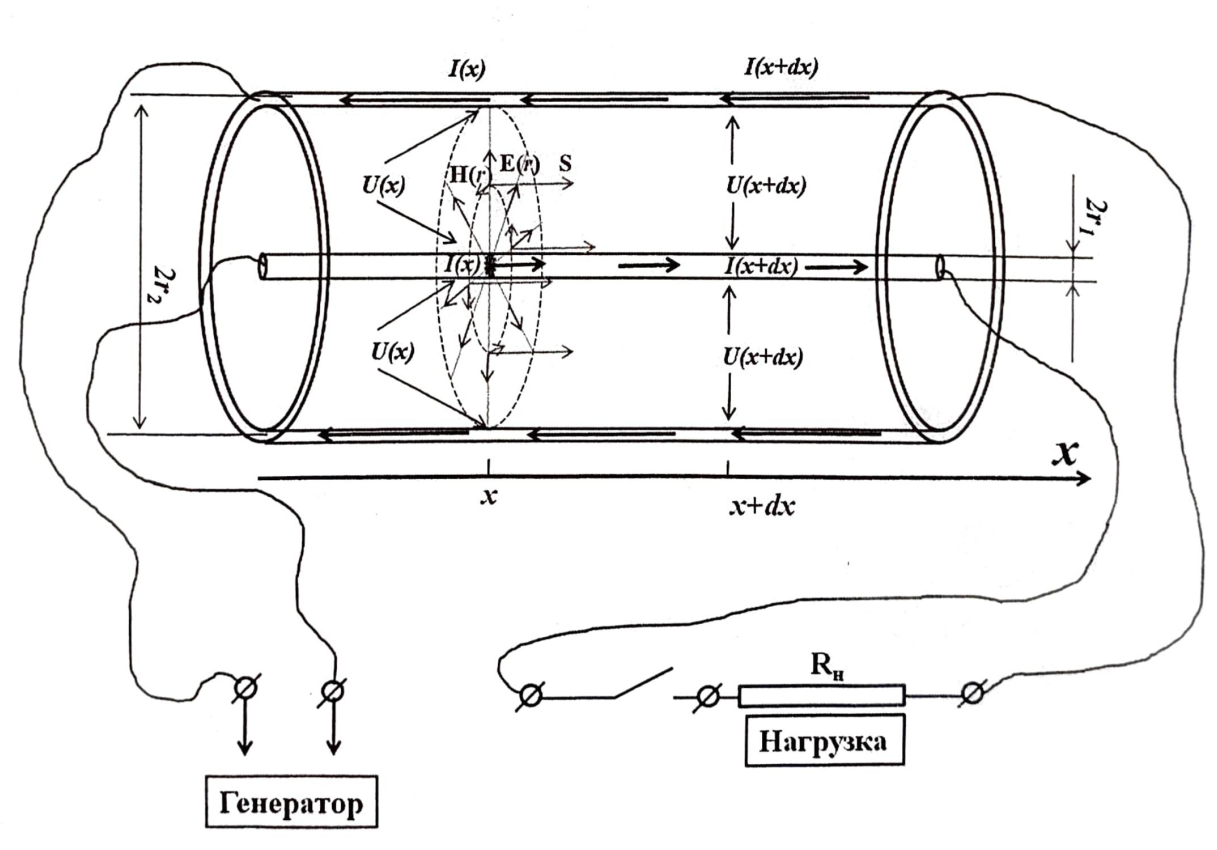
\includegraphics[scale=0.4]{figures/2024-10-24_22-17.png}
\end{figure}
В данной работе сигналы передаются по длинному коаксиальному кабелю, который
представляет из себя систему двух проводников -- изолированный коаксиальный
медный проводящий цилиндр радиуса $r_2$ и тонкий медный проводник, имеющий
радиус $r_1$ и расположенный на оси цилиндра. Пространство между ними заполнено
веществом, имеющим диэлектрическую проницаемость $\varepsilon$ и магнитную
восприимчивость $\mu$.

Рассмотрим элемент $dx$ такого кабеля. Такой элемент обладает индуктивностью
\begin{equation}
	dL=2\mu\ln\left(\frac{r_2}{r_1}\right)dx
\end{equation}
\begin{equation}
	L_x=\dv{x}{L}=2\mu\ln\left(\frac{r_2}{r_1}\right)
\end{equation}
величина $L_x$ называется погонной индуктивностью.

Так же два проводника обладают взаимной ёмкостью
\begin{equation}
	dC=\frac{\varepsilon}{2\ln(r_2/r_1)}dx
\end{equation}
аналогично определяется погонная ёмкость
\begin{equation}
	C_x=\dv{x}{C}=\frac{\varepsilon}{2\ln(r_2/r_1)}
\end{equation}
При передаче сигналов по такому
кабелю возникают противоположно направленные токи по внешней оболочке и
внутреннему проводнику, а также напряжение между проводниками. При высоких
частотах величины $I$ и $U$ будут зависеть от $x$.

Падение напряжения на концах выбранного элемента связано с возникновением ЭДС
индукции и омическим сопротивлением.
\begin{equation}\label{Ueq}
	U(x+dx)-U(x)=-\frac{L_xdx}{c^2}\frac{\partial I}{\partial t}-R_xIdx
\end{equation}
\begin{equation}
	R_x = \dv{x}{R} = \frac{1}{\sigma S}
\end{equation}
где $R_x$ -- погонное сопротивление, $\sigma$ --
удельная проводимость, $S=\pi r_1^2$ -- площадь поперечного сечения проводника.

Изменение силы тока связано с перетеканием части заряда на ёмкость, т.е
\begin{equation}\label{Ieq}
	I(x+dx)-I(x)=-\frac{\partial q}{\partial t}=-C_x dx \frac{\partial U}{\partial t}
\end{equation}

Разделив уравнения \eqref{Ueq} и \eqref{Ieq} на $dx$ и
продифференцировав первое уравнение по $x$, а второе по $t$
получим систему.
\begin{equation}\label{WaveSystUeq}
	\begin{cases}
		\frac{\partial^2 U}{\partial x^2}=-\frac{L_x}{c^2}\frac{\partial I}{\partial x\partial t}-R_x\frac{\partial I}{\partial x}
		\\
		\frac{\partial I}{\partial t\partial x}=-C_x\frac{\partial^2 U}{\partial t^2}
	\end{cases}
\end{equation}
Итого получим уравнение
\begin{equation}\label{WaveUeq}
	\frac{\partial^2 U}{\partial t^2}-V^2_\text{ф}\frac{\partial^2 U}{\partial x^2}+\gamma\frac{\partial U}{\partial t}=0
\end{equation}
\begin{equation}
	V_\Phi=\frac{c}{\sqrt{L_xC_x}}
\end{equation}
\begin{equation}
	\gamma=R_xC_xV^2_\text{ф}
\end{equation}
где $V_\text{ф}$ -- фазовая скорость,
$\gamma$ -- декремент затухания.\\
Подставив погонные
характеристики в выражение для фазовой скорости, заметим, что фазовая скорость
совпадает со скоростью распространения электромагнитных волн в среде.

\begin{equation}
	V_\text{ф}=\frac{c}{\sqrt{\varepsilon\mu}}
\end{equation}

Решение уравнения \eqref{WaveUeq} ищется в виде
\begin{equation}\label{WaveUsol}
	U(x,t)=U_0e^{-i\omega t}e^{(-\alpha+ik)x} \implies
\end{equation}
\begin{equation}\label{alphaSol}
	\alpha=\frac{\omega}{V_\text{ф}}\sqrt{\frac{\sqrt{1+(\gamma/\omega)^2}-1}{2}}\approx
	\frac{\omega}{V_\text{ф}}\sqrt{\frac{\gamma^2}{4\omega^2}}=
	\frac{\gamma}{2V_\text{ф}}=R_xC_x\frac{V_\text{ф}}{2}
\end{equation}

\begin{equation}\label{kSol}
	k=\frac{\omega}{V_\text{ф}}
\end{equation}

\begin{equation}\label{Un}
	U_\text{н}(t)=U_0e^{-\alpha l}e^{ikl}e^{-\omega t}
\end{equation}

При этом амплитуда колебаний на согласованной нагрузке (в конце длинной линии) имеет вид:
\begin{equation}\label{UnAmp}
	U_\text{н}=U_0e^{-\alpha l}
\end{equation}
Так же получена разность фаз
\begin{equation}\label{dphi}
	\Delta \varphi=kl
\end{equation}

Из уравнений \eqref{UnAmp} и \eqref{dphi} получим соотношения для экспериментального определения $\alpha$ и $k$ для различных $\omega$

\begin{equation}\label{alphaomega}
	\alpha(\omega)=\frac{1}{l}\ln\frac{U_0}{U_\text{н}}
\end{equation}

\begin{equation}\label{komega}
	k(\omega)=\frac{\Delta \varphi}{l}
\end{equation}

\begin{equation}\label{k}
	\omega=k V_\Phi
\end{equation}

\subsection{Экспериментальная установка}
Коаксиальный кабель подключается к генератору и осциллографу. На канал 1
выводится сигнал, подаваемый генератором, а с канала 2 снимается напряжение на
нагрузке. Схема экспериментальной установки изображена ниже.

\section{Ход работы.}

Соберем схему согласно рис. \ref{fig:s1}
\begin{figure}[H]
	\centering
	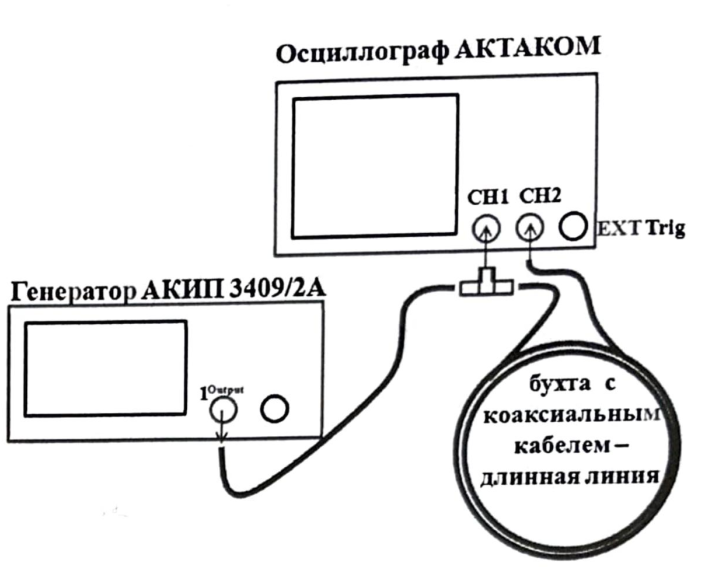
\includegraphics[scale=0.5]{figures/s1.png}
	\caption{Схема для установки наблюдения распространения сигналов вдоль длинной линии.}
	\label{fig:s1}
\end{figure}
Ознакомимся с осциллографом и генератором.

\subsection{Согласованная линия.}
\begin{enumerate}
	\item Выставим сопротивление на осциллографе $ 50 \Ohm $.
	\item \label{p:1.2} Пронаблюдаем, как меняется сигнал на осциллографе при $ \nu \in [1 \mega\Hz, 30 \mega\Hz] $.
	\item \label{p:1.3} Определим резонансные частоты.
	      Из ур-ия \ref{komega}:
	      \begin{gather}
		      k = \frac{2\pi n}{l} \implies \\
		      \nu_n = \frac{V_\Phi}{l} n
	      \end{gather}
	      \begin{table}[H]
		      \centering
		      \begin{tabular}{|l|l|l|l|l|l|l|l|}
			      \hline
			      $ \nu_n, \mega\Hz $ & 3.9 & 7.9 & 11.9 & 15.9 & 19.9 & 23.8 & 27.8 \\
			      \hline
		      \end{tabular}
	      \end{table}
	\item \label{p:1.4} Найдем фазовую частоту $ V_\Phi $.\\
	      Найдем наклон прямой $ \nu(n) $.
	      \begin{equation}
		      \frac{V_\Phi}{l} \approx 4 \mega\Hz
	      \end{equation}
	      \[
		      l = 50.1 \m
		      .\]
	      \begin{equation}
		      V_\Phi \approx 2 \cdot 10^{8} \cdot \m \cdot \Hz
	      \end{equation}
\end{enumerate}
\subsection{Линия без нагрузки.}
\begin{enumerate}
	\setcounter{enumi}{4}
	\item Выставим сопротивление на осциллографе $ 1 \mega\Ohm $.
	      Выполним пункты \ref{p:1.2} и \ref{p:1.4}.
	\item
	\item
	      \begin{table}[H]
		      \centering
		      \begin{tabular}{|l|l|l|l|l|l|l|l|}
			      \hline
			      $ \nu_n, \mega\Hz $ & 3.98 & 7.98 & 11.98 & 15.87 & 19.96 & 23.97 & 27.98 \\
			      \hline
		      \end{tabular}
	      \end{table}
	\item
	      \begin{equation}
		      \frac{V_\Phi}{l} \approx 4 \mega\Hz
	      \end{equation}
	      \begin{equation}
		      V_\Phi \approx 2 \cdot 10^{8} \cdot \m \cdot \Hz
	      \end{equation}
\end{enumerate}
\subsection{Прямоугольные импульсы.}
\begin{enumerate}
	\item Выставим сопротивление на осциллографе $ 50 \Ohm $.
	\item[2-3.] \label{p:3:2} Настроим генератор согласно указаниям.
	      \setcounter{enumi}{3}
	\item Меняя параметры генератора пронаблюдаем изменение сигнала на осциллографе.
	\item Вернем параметры согласно п. 2 (\ref{p:3:2}).
	\item Определим резонансные частоты при $ \nu \in [1 \mega\Hz, 20 \mega\Hz] $.
	      \begin{table}[H]
		      \centering
		      \begin{tabular}{|l|l|l|l|l|l|l|l|}
			      \hline
			      $ \nu_n, \mega\Hz $ & 4 & 8 & 12 & 16 & 20 & 24 & 28 \\
			      \hline
		      \end{tabular}
	      \end{table}
	\item
	      \begin{equation}
		      \frac{V_\Phi}{l} \approx 4 \mega\Hz
	      \end{equation}
	      \begin{equation}
		      V_\Phi \approx 2 \cdot 10^{8} \cdot \m \cdot \Hz
	      \end{equation}
\end{enumerate}

\subsection{АЧХ и ФЧХ.}
\begin{enumerate}
	\item Выставим сопротивление на осциллографе $ 50 \mega\Ohm $.
	      Выполним пункты \ref{p:1.2} и \ref{p:1.4}.
	\item [2-4.] Настроим генератор согласно указаниям.
	      \setcounter{enumi}{4}
	\item При $ \mu \in [1 \mega\Hz, 40 \mega\Hz] $ снимим АЧХ и ФЧХ.
	      (см. т. \ref{table:АЧХ_ФЧХ})
	      \begin{table}[H]
		      \centering
		      \begin{tabular}{|l|l|l|}
			      \hline
			      $\nu, \mega\Hz$ & $U, \Volt$ & $\Delta \varphi, \nano\sec$ \\
			      \hline
			      1               & 25         & 250.0                       \\
			      3               & 24         & 78.0                        \\
			      5               & 23         & 53.6                        \\
			      7               & 23         & 33.6                        \\
			      8               & 23         & 31.2                        \\
			      11              & 22         & 21.0                        \\
			      13              & 22         & 21.2                        \\
			      16              & 21         & 1.3                         \\
			      19              & 21         & 12.1                        \\
			      22              & 21         & 21.8                        \\
			      25              & 20         & 10.7                        \\
			      30              & 19         & 15.8                        \\
			      35              & 18         & 6.7                         \\
			      40              & 17         & 0.7                         \\
			      \hline
		      \end{tabular}
		      \label{table:АЧХ_ФЧХ}
		      \caption{АЧХ и ФЧХ}
	      \end{table}
\end{enumerate}

\subsection{Обработка результатов измерений.}
\paragraph{Часть I. Определение параметров коаксиального кабеля.}
\begin{equation}
	y_1 = \frac{L_x C_x}{c^2} x_1
\end{equation}
\begin{gather}
	x_1 = \omega^2 \\
	y_1 = k^2 - \alpha^2
\end{gather}
\begin{gather*}
	k = \frac{\Delta \varphi}{l} \\
	\alpha = \frac{1}{l} \ln{\frac{U_0}{U_\text{н}}}
\end{gather*}

\begin{figure}[H]
	\centering
	\includesvg[width=0.9\linewidth]{figures/y1(x1).svg}
\end{figure}


\begin{table}[H]
	\centering
	\begin{tabular}{|l|l|l|}
		\hline
		$\nu, \mega\Hz$ & $U, \Volt$ & $\Delta{\varphi}, \rad$ \\
		\hline
		1               & 25         & 3                       \\
		3               & 24         & 4                       \\
		5               & 23         & 7                       \\
		7               & 23         & 8                       \\
		8               & 23         & 10                      \\
		11              & 22         & 12                      \\
		13              & 22         & 15                      \\
		16              & 21         & 20                      \\
		19              & 21         & 22                      \\
		22              & 21         & 25                      \\
		25              & 20         & 30                      \\
		30              & 19         & 37                      \\
		35              & 18         & 42                      \\
		40              & 17         & 50                      \\
		\hline
	\end{tabular}
	\hspace{1cm}
	\begin{tabular}{|l|l|}
		\hline
		$x_1, 10^{14} / \sec^2$ & $y_1, 10^{-2} / \m^2$ \\
		\hline
		0                       & 0                     \\
		4                       & 1                     \\
		10                      & 2                     \\
		19                      & 3                     \\
		25                      & 4                     \\
		48                      & 6                     \\
		67                      & 9                     \\
		101                     & 16                    \\
		143                     & 20                    \\
		191                     & 24                    \\
		247                     & 35                    \\
		355                     & 54                    \\
		484                     & 71                    \\
		632                     & 101                   \\
		\hline
	\end{tabular}
\end{table}

Наклон:
\[
	a = (15 \pm 1) \cdot 10^{-18} \frac{\sec^2}{\m^2}
\]
\[
	L_x C_x = 1.4 \pm 0.1
\]
Знаем $R_0 = 50 \Ohm$.
$$
	R_0 = \frac{1}{c} \sqrt{\frac{L_x}{C_x}}
$$
$$
	L_x^2 = (L_x C_x) R_0^2 c^2, \quad C_x = \frac{(L_x C_x)}{L_x}
$$
$$
	L_x = (2.0 \pm 0.1)\ \eaCGS
$$
$$
	C_x = (0.7 \pm 0.1)\ \eaCGS
$$
$$
	V_\Phi = \frac{c}{\sqrt{L_x C_x}} = (2.54 \pm 0.08) \cdot 10^{10}\ \eaCGS
$$
$$
	2 \ln\frac{r_2}{r_1} \approx 2.14
$$
$$
	\varepsilon = 2 \ln\frac{r_2}{r_1} C_x = (1.5 \pm 1) \eaCGS
$$
$$
	\mu = \frac{L_x}{2 \ln\frac{r_2}{r_1}} = (0.9 \pm 0.1) \eaCGS
$$

\paragraph{Часть II. Определение удельной проводимости проводников.}
\subparagraph{Метод A.} \\

Построим график $y_2(x_2)$, где
\Cases{
	x_2 = \sqrt{\nu} \\
	y_2 = \alpha(\omega) = \frac{4 C_x V_\Phi}{\sqrt{\sigma} d c} \cdot x_2
}\\
$$
	a = \Delta y_2 / \Delta x_2
$$
$$
	\sigma = \left(\frac{2 C_x V_\Phi}{c d a}\right)^2
$$
\begin{table}[H]
	\centering
	\begin{tabular}{|l|l|}
		\hline
		$x_2, 10^{3} / \sqrt\sec$ & $y_2, 10^{-3} / \m^2$ \\
		\hline
		1.0                       & 0.4                   \\
		1.7                       & 1.0                   \\
		2.2                       & 1.8                   \\
		2.6                       & 2.0                   \\
		2.8                       & 2.1                   \\
		3.3                       & 2.6                   \\
		3.6                       & 2.9                   \\
		4.0                       & 3.2                   \\
		4.4                       & 3.5                   \\
		4.7                       & 3.9                   \\
		5.0                       & 4.6                   \\
		5.5                       & 5.2                   \\
		5.9                       & 6.1                   \\
		6.3                       & 6.6                   \\
		\hline
	\end{tabular}
\end{table}
\begin{figure}[H]
	\centering
	\includesvg[width=0.9\linewidth]{figures/y2(x2).svg}
\end{figure}
$$
	a = (1.13 \pm 0.7) \cdot 10^{-8}\ \eaCGS
$$
$$
	d = 1.37 \m
$$
$$
	\sigma = (61 \pm 6) \cdot 10^{16}\ \eaCGS
$$
\subparagraph{Метод B.}
Построим график $y_2(x_2)$, где
\Cases{
	x_3 = \nu^{\frac{3}{2}} \\
	y_2 = \alpha(\omega) k(\omega)
}\\
$$
	a = \Delta y_3 / \Delta x_3
$$
$$
	\sigma = \left(\frac{4 \pi C_x}{c d a}\right)^2
$$
\begin{table}[H]
	\centering
	\begin{tabular}{|l|l|}
		\hline
		$x_3, 10^{9} / \sec^{\frac{3}{2}}$ & $y_3, 10^{-3} / \m^4$ \\
		\hline
		1                                  & 0.0                   \\
		5                                  & 0.1                   \\
		11                                 & 0.2                   \\
		19                                 & 0.3                   \\
		23                                 & 0.4                   \\
		36                                 & 0.6                   \\
		47                                 & 0.8                   \\
		64                                 & 1.3                   \\
		83                                 & 1.5                   \\
		103                                & 1.9                   \\
		125                                & 2.7                   \\
		164                                & 3.8                   \\
		207                                & 5.1                   \\
		253                                & 7.0                   \\
		\hline
	\end{tabular}
\end{table}
\begin{figure}[H]
	\centering
	\includesvg[width=0.9\linewidth]{figures/y3(x3).svg}
\end{figure}
$$
	a = (26 \pm 1) \cdot 10^{-19}\ \eaCGS
$$
$$
	d = 1.37 \m
$$
$$
	\sigma = (68 \pm 6) \cdot 10^{10}\ \eaCGS
$$
Табличное значение:
$$
	\sigma_0 \approx 60 \cdot 10^6 \frac{\text{См}}{\m}
	=\ ?\ \eaCGS \approx 60 \cdot 10^{16}\ \eaCGS
$$
\section{Длинная линия. Модель.}

Определим предельную частоту распространения
сигнала
$v_0 = 1/\pi\sqrt{LC} = 38 \kilo\Hz$, согласованную нагрузку
$R_0 = \sqrt{L/C} = 178 \Ohm$.

\begin{table}[H]
	\centering
	\begin{tabular}{|c|c|c|c|c|c|c|c|c|c|c|} \hline
		$\nu, \kilo\Hz$  & 1 & 3  & 5  & 8  & 10 & 15 & 20  & 25  & 30  & 35  \\
		\hline
		$\Delta \varphi$ & 6 & 17 & 31 & 52 & 63 & 93 & 122 & 160 & 186 & 218 \\
		\hline
	\end{tabular}
	\caption{Данные  по длинной волне}
\end{table}

\begin{figure}[H]
	\centering
	\includesvg[width=0.9\linewidth]{figures/g1.svg}
\end{figure}
$$
	a = \Delta y / \Delta x = (6.2 \pm 0.1) \ \mili\sec
$$
% $$
% \Delta \varphi = 2\pi \frac{l}{V_\Phi} \nu
% $$
% $\frac{V_\Phi}{l} \approx 4 \kilo\Hz$
% $\frac{l}{V_\Phi} \approx 0.25 \cdot 10^{-3} \sec$
%
% Из теоретических формул можно вывести, что коэфицент наклона графика должен
% быть равен $2\pi/\epsilon_0$ = 5.96*$10^{-3}c^{-2}.$ Построим график и получим
% свой коэфицент наклона.

\begin{table}[H]
	\centering
	\begin{tabular}{|c|c|c|c|c|c|c|c|c|c|c|} \hline
		$N$              & 1 & 2  & 3  & 4  & 5  & 6  & 7   & 8   & 9   & 10  \\
		\hline
		$U, \Volt$ & 47 & 30 & 12 & 30 & 45 & 48 & 34 & 9 & 21 & 41 \\
		\hline
	\end{tabular}
	\caption{Данные  по длинной волне}
\end{table}

Построим график зависимости напряжения между ячейками
от номера при $\nu = 9.8 \kilo\Hz$.
\begin{figure}[H]
	\centering
	\includesvg[width=0.9\linewidth]{figures/U.svg}
\end{figure}

\section{Вывод.}
В ходе данной лабораторной работы мы ознакомились и проверили теорию распространения
электрических сигналов вдоль длинной линии.
Нашли $V_\Phi, L_x, C_x, \varepsilon, \mu$.
$$
	L_x = (2.0 \pm 0.1)\ \eaCGS
$$
$$
	C_x = (0.7 \pm 0.1)\ \eaCGS
$$
$$
	V_\Phi = (2.54 \pm 0.08) \cdot 10^{10}\ \eaCGS
$$
$$
	\varepsilon = (1.5 \pm 0.1) \eaCGS
$$
$$
	\mu = (0.9 \pm 0.1) \eaCGS
$$
Сняли АЧХ и ФЧХ.
Нашли $\sigma$ двумя способами.
$$
	\sigma_1 = (61 \pm 6) \cdot 10^{16}\ \eaCGS
$$
$$
	\sigma_2 = (68 \pm 6) \cdot 10^{10}\ \eaCGS
$$
$\sigma_1$ похоже на табличное значение.

\end{document}
